\subsection{滤过环与滤过模}

定义 1. 一个递增（相应地，递减）序列 \((\mathbf{G}_n)_{n\in \mathbf{Z}}\) （由群 \(\mathbf{G}\) 的子群组成）称为 \(\mathbf{G}\) 上的一个递增（相应地，递减）滤过。

带有一个滤过的群称为滤过群。

若 \((\mathrm{G}_{n})_{n\in\mathbf{Z}}\) 是群 G 上的一个递增（相应地，递减）滤过，并且记 \(G_{n}^{\prime}=G_{-n}\) ，则显然 \((\mathrm{G}_{n}^{\prime})_{n\in\mathbf{Z}}\) 是 G 上的一个递减（相应地，递增）滤过。因此我们可以把研究局限于递减滤过，今后凡谈到滤过，除另有说明外，均指递减滤过。

设 \((\mathbf{G}_n)_{n\in \mathbf{Z}}\) 是群 \(\mathbf{G}\) 上的一个递减滤过，显然 \(\bigcap_{n\in \mathbf{Z}}\mathbf{G}_n\) 与 \(\bigcup_{n\in \mathbf{Z}}\mathbf{G}_n\) 都是 \(\mathbf{G}\) 的子群；若 \(\bigcap_{n\in \mathbf{Z}}\mathbf{G}_n\) 化为单位元，则称该滤过是分离的；若 \(\bigcup_{n\in \mathbf{Z}}\mathbf{G}_n = \mathbf{G}\) ，则称它是穷竭的。

定义 2. 给定环 A，加法群 A 上的滤过 \((\mathbf{A}_n)_{n\in \mathbf{Z}}\) 称为与 A 的环结构相容，如果

\[
\mathrm{A} _ {m} \mathrm{A} _ {n} \subset \mathrm{A} _ {m + n} \quad for \quad m \in \mathbf {Z}, \quad n \in \mathbf {Z}\tag{1}
\]

\[
\mathbf {1} \in \mathbf {A} _ {0}.\tag{2}
\]

带有这个滤过的环 A 称为滤过环。

条件 (1) 与 (2) 表明 \(\mathbf{A}_0\) 是 \(\mathbf{A}\) 的子环，且诸 \(\mathbf{A}_n\) 是（左与右）\(\mathbf{A}_0\) -模。集合 \(\mathbf{B} = \bigcup_{n \in \mathbf{Z}} \mathbf{A}_n\) 是 \(\mathbf{A}\) 的子环，而集合 \(\mathfrak{n} = \bigcap_{n \in \mathbf{Z}} \mathbf{A}_n\) 是 \(\mathbf{B}\) 的双边理想；因为若 \(x \in \mathfrak{n}\) 且 \(a \in \mathbf{A}_p\) ，则对一切 \(k \in \mathbf{Z}\) 有 \(x \in \mathbf{A}_{k-p}\) ，于是由 (1) 得 \(ax \in \mathbf{A}_k\) 且 \(xa \in \mathbf{A}_k\) ；因而 \(ax \in \mathfrak{n}\) 且 \(xa \in \mathfrak{n}\) 。

一个重要的特殊情形是 \(\mathbf{A}_0 = \mathbf{A}\) 的情形；这时 \(\mathbf{A}_n = \mathbf{A}\) 对 \(n \leqslant 0\) 成立，并且所有 \(\mathbf{A}_n\) 都是 \(\mathbf{A}\) 的双边理想。

定义 3. 设 A 是一个滤过环，\((\mathbf{A}_n)_{n\in \mathbb{Z}}\) 是它的滤过，E 是一个 A-模。E 上的滤过 \((\mathrm{E}_n)_{n\in \mathbb{Z}}\) 称为与 E 在滤过环 A 上的模结构相容，如果

\[
\mathrm{A} _ {m} \mathrm{E} _ {n} \subset \mathrm{E} _ {m + n} \quad for \quad m \in \mathbf {Z}, \quad n \in \mathbf {Z}.\tag{3}
\]

带有这个滤过的 A-模 E 称为滤过模。

诸 \(\mathbf{E}_n\) 都是 \(\mathbf{A}_0\) -模；若 \(\mathbf{B} = \bigcup_{n \in \mathbf{Z}} \mathbf{A}_n\) ，显然 \(\bigcup_{n \in \mathbf{Z}} \mathbf{E}_n\) 是一个 B-模，且 \(\bigcap_{n \in \mathbf{Z}} \mathbf{E}_n\) 由上面关于 \(\bigcap_{n \in \mathbf{Z}} \mathbf{A}_n\) 的同样论证也是一个 B-模。若 \(\mathbf{A}_0 = \mathbf{A}\) ，则所有 \(\mathbf{E}_n\) 都是 \(\mathbf{E}\) 的子模。

\textbf{例}\par

\begin{enumerate}
\def\labelenumi{(\arabic{enumi})}
\tightlist
\item
  设 A 是一个 Z 型分次环；对一切 \(i \in Z\) ，用 \(\mathbf{A}_{(i)}\) 表示 A 中次数为 i 的齐次元组成的子群。记 \(A_{n} = \sum_{i \geq n} A_{(i)}\) ；则立即可见 \((\mathbf{A}_{n})\) 是一个与 A 的环结构相容的、穷竭且分离的递减滤过；称这个滤过为与分次 \((\mathbf{A}_{(i)})_{i \in \mathbf{Z}}\) 相伴的滤过，称滤过环 A 为与给定的分次环 A 相伴的滤过环。
\end{enumerate}

现在设 E 是分次环 A 上的一个 Z 型分次模，对一切 \(i \in Z\) ，用 \(\mathrm{E}_{(i)}\) 表示 E 中次数为 i 的齐次元组成的子群。记 \(\mathrm{E}_{n} = \sum_{i \geqslant n} \mathrm{E}_{(i)}\) ；则 \((\mathrm{E}_{n})\) 是一个穷竭且分离的递减滤过，它与 E 在滤过环 A 上的模结构相容；称这个滤过为与分次 \((\mathrm{E}_{(i)})_{i \in \mathbf{Z}}\) 相伴的滤过，称滤过模 E 为与给定的分次模 E 相伴的滤过模。(2) 设 A 是一个滤过环，\((\mathrm{A}_{n})_{n \in \mathbf{Z}}\) 是它的滤过，E 是一个 A-模。记 \(E_{n} = A_{n}E\) ；由 (1) 推出

\[
\mathbf {A} _ {m} \mathbf {E} _ {n} = \mathbf {A} _ {m} \mathbf {A} _ {n} \mathbf {E} \subset \mathbf {A} _ {m + n} \mathbf {E} = \mathbf {E} _ {m + n},
\]

并由 (2) 推出 \(E_{0} = E\) ；于是 \((\mathrm{E}_{n})\) 是一个与 E 的 A-模结构相容的穷竭滤过。称这个滤过为由 A 上给定的滤过 \((\mathrm{A}_{n})\) 导出的滤过；注意它未必是分离的，即使 \((\mathbf{A}_n)\) 是分离的，且 \(\mathbf{E}\) 与诸 \(\mathbf{A}_n\) 都是有限生成的 A-模（参看 § 3 习题 2；不过可参看 § 3 第 3 节命题 5 以及第 2 节命题 4 的推论）。

\begin{enumerate}
\def\labelenumi{(\arabic{enumi})}
\setcounter{enumi}{2}
\tightlist
\item
  设 A 是一个环，m 是 A 的一个双边理想。记 \(A_{n} = m^{n}\) （ \(n \geqslant 0\) ），\(A_{n} = A\) （n \textless{} 0）；立即可见 \((\mathbf{A}_{n})\) 是 A 上的一个穷竭滤过，称为 m-进滤过。设 E 是一个 A-模；由 A 上的 m-进滤过导出的 E 的滤过 \((\mathbf{E}_{n})\) 称为 E 上的 m-进滤过；换言之，\(E_{n} = m^{n}E\) （ \(n \geqslant 0\) ），\(E_{n} = E\) （n \textless{} 0）。
\end{enumerate}

若 A 是交换的且 B 是一个 A-代数，则 n = mB 是 B 的双边理想，并且对每个 B-模 F 有 \(n^{k}F = m^{k}F\) ，因此 F 上的 n-进滤过与 m-进滤过一致（若把 F 看作 A-模）。

\begin{enumerate}
\def\labelenumi{(\arabic{enumi})}
\setcounter{enumi}{3}
\item
  若 A 是一个滤过环，\((\mathbf{A}_{n})\) 是它的滤过，则左 A-模 \(A_{s}\) 带有滤过 \((\mathbf{A}_{n})\) 而是一个滤过 A-模。另一方面，显然 \((\mathbf{A}_{n})\) 是一个与反环 \(A^{0}\) 的环结构相容的滤过，且 \(A_{d}\) 是一个滤过（左）\(A^{0}\) -模，带有滤过 \((\mathbf{A}_{n})\) 。
\item
  在环 A 上，诸集合 \(A_{n}\) ，其中 \(A_{n}=0\) （n\textgreater0），\(A_{n}=A\) （ \(n\leqslant0\) ），构成所谓 A 上的平凡滤过，即与 A 上的平凡分次相伴的滤过（例 1）；在 A-模 E 上，凡由 A-子模组成的滤过 ( \(E_{n}\) ) 都与 E 在滤过环 A 上的模结构相容。于是可以说，每个滤过交换群 G 都是一个滤过 Z-模，只要给 Z 赋以平凡滤过。
\end{enumerate}

设 \(G\) 是一个滤过群，\((G_n)_{n \in \mathbf{Z}}\) 是它的滤过；显然，若 \(H\) 是 \(G\) 的任意一个子群，则 \((H \cap G_n)_{n \in \mathbf{Z}}\) 是一个滤过，称为由 \(G\) 上的滤过诱导的诱导滤过；若 \(G\) 上的滤过是穷竭的（相应地，分离的），则它也是。类似地，若 \(H\) 是 \(G\) 的一个正规子群，则族 \(((H.G_n)/H)_{n \in \mathbf{Z}}\) 是群 \(G/H\) 上的一个滤过，称为关于 \(H\) 的商滤过（\(G\) 上的滤过的商）；若 \((G_n)\) 是穷竭的，则它也是。若 \(G'\) 是另一个滤过群，\((G_n')_{n \in \mathbf{Z}}\) 是它的滤过，则 \((G_n \times G_n')\) 是 \(G \times G'\) 上的一个滤过，称为 \(G\) 与 \(G'\) 上的滤过的乘积滤过；若 \((G_n)\) 与 \((G_n')\) 都是穷竭的（相应地，分离的），则它也是。

现在设 A 是一个滤过环，\((\mathbf{A}_{n})\) 是它的滤过；在 A 的每个子环 B 上，显然由 A 上的滤过诱导的滤过与 B 的环结构相容。若 b 是 A 的一个双边理想，则 A 上的滤过在 A/b 上的商滤过与这个环的结构相容，因为

\[
\left(\mathrm{A} _ {n} + \mathfrak {b}\right) \left(\mathrm{A} _ {m} + \mathfrak {b}\right) \subset \mathrm{A} _ {n + m} + \mathfrak {b}.
\]

若 \(A'\) 是另一个滤过环，则 \(A \times A'\) 上的乘积滤过与这个环的结构相容。

最后设 E 是一个滤过 A-模，\((E_{n})\) 是它的滤过；在 E 的每个子模 F 上，由 E 上的滤过诱导的滤过与 F 的 A-模结构相容，而在商模 E/F 上，E 上的滤过的商滤过与 A-模结构相容，因为

\[
\mathrm{A} _ {n} (\mathrm{F} + \mathrm{E} _ {m}) \subset \mathrm{F} + \mathrm{A} _ {n} \mathrm{E} _ {m} \subset \mathrm{F} + \mathrm{E} _ {m + n}.
\]

\pandocbounded{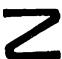
\includegraphics[keepaspectratio]{images/part002_676c5d74.jpg}}

注意，若 E 上的滤过是由 A 上的滤过导出的（例 2），则 E/F 上的商滤过也是，但 F 上诱导的滤过一般不是（习题 1；不过可参看 § 3 第 2 节定理 2）。

若 \(E'\) 是另一个滤过 A-模，则 \(E \times E'\) 上的乘积滤过与它的 A-模结构相容。若 E 与 \(E'\) 上的滤过都是由 A 上的滤过导出的（例 2），则它们的乘积滤过也是。
% semantic-fragments: legacy-input-seam
\relax{}
